\chapter{Présentation de la structure de formation}
\markboth{Chapitre 1. Présentation de la structure de formation}{} 
\begin{spacing}{1.2}
\minitoc
\thispagestyle{MyStyle}
\end{spacing}
\newpage

\section*{Introduction}
Dans ce chapitre il sera question de présenter l’Université Norbert ZONGO, l’Unité de Recherche et de Formation Sciences et Technologie qui est notre structure de formation, et présenter le cadre de notre stage à la Direction des Services Informatique de l’université.
\section{Présentation de l’Université Norbert Zongo}
Créée par décret N° 2005-460/PRES/PM/ MESSRS/MFB le 31 août 2005, suite à la transformation de l’École normale supérieure de Koudougou (ENSK)\cite{infoUNZbf}.

\par L’Université Norbert ZONGO était appelé Université de Koudougou de sa création jusqu’au 30 novembre 2017 où elle fût renommée en hommage au journaliste d'investigation Norbert Zongo par décret pris en conseil des ministres du 27 juillet de la même année. \cite{infoUNZbf}
 
\par Située à Koudougou, troisième ville du pays, chef-lieu de la province du Boulkiemdé et de la région du Centre-Ouest L’UNZ s’étend sur une superficie de 200 hectares attribué par les arrêtés n°2005-03/MATD/SG/PBLK/CKDG du 14 avril 2005 et n°2005-05/MATD/SG/PBLK/CKDG du 24 juin 2005 \cite{infoUNZbf}.
\par

Les différents responsables ont été:

\textbf{Dr Mathieu R. OUEDRAOGO}, directeur général de l’ENSK de sept 1996 à novembre 1998;\\

\textbf{Pr Amadé BADINI}, directeur général de l’ENSK de novembre 1998 à décembre 2003;\\

\textbf{Pr Bila Gérard SEGDA}, directeur général de l’ENSK de décembre 2003 à août 2005 et président de l’Université de Koudougou d’août 2005 au 6 mars 2013 ;\\

\textbf{Pr Georges SAWADOGO}, président de l’Université de Koudougou du 2 avril 2013 au 17 mai 2017;\\

\textbf{Pr Nicolas BARRO}, président de l’Université de Koudougou du 17 mai 2017 au 30 novembre 2017 puis président de l’Université Norbert ZONGO jusqu’au 6 juin 2019;\\

\textbf{Pr Frédéric OUATTARA} président de l’Université Norbert ZONGO depuis le 6 juin 2019;

\textbf{Pr Issa Abdou MOUMOULA} président de l’Université Norbert ZONGO depuis le 5 mai 2022. \par
Sa devise est "Scientia Excelle Ut Melius Servias" ce qui signifie : Exceller par le Savoir pour mieux Servir.
L’UNZ compte aujourd’hui un institut et trois UFR listée dans le tableau suivant.
\begin{table}[h]
  \begin{tabular}{ |p{5cm}|p{5cm}|p{5cm}| }
\hline
\multicolumn{3}{|c|}{Liste des unités de formation et de recherche} \\
\hline
UFR LSH & UFR SEG & UFR ST \\
\hline
Géographie & APE & MPCI\\
Lettres Modernes & EAE & Mathématiques \\
Psychologie & ESG & Physique  \\
Histoire et archéologie &   & Chimie  \\
Philosophie &   & Informatique  \\
SID &   &  SVT \\
    &   &  Sciences biologiques \\
    &   &  Biochimie \\
\hline
\end{tabular}

  \caption{Unités de formation de l'Université Norbert ZONGO}
  \label{tab:Unités de formation de l'Université Norbert ZONGO}
\end{table}

\section{Présentation de l’UFR ST}
Dans le but de former les étudiants dans les domaines scientifiques et technologiques L’UFR ST a été créée en 2014 avec divers une offre de formation.
L’UFR ST est actuellement sous la direction du Dr Arouna OUEDRAOGO. Elle  renferme les filières scientifiques telle que MPCI et SVT dont les premières années se font en tronc commun avant l’entame d’un parcoure plus précis. 

\begin{figure}[H]%
    \center%
    \setlength{\fboxsep}{5pt}%
    \setlength{\fboxrule}{0.5pt}%
    \fbox{
    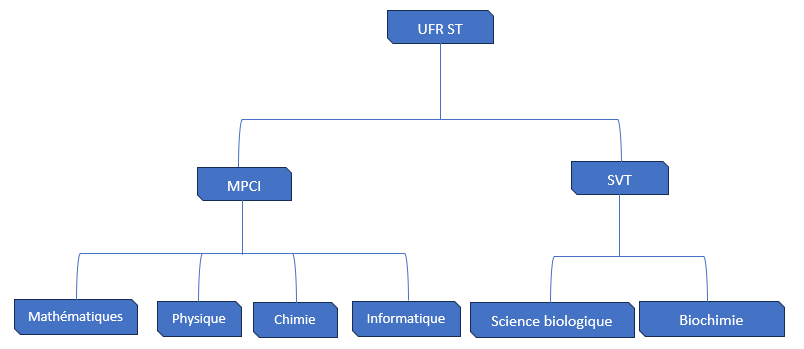
\includegraphics[width=16cm,height=9cm]{images/organigramme st.PNG}%
    }
    \caption{Organigramme des filières de l'UFR ST}%
\end{figure}


\section{Cadre de stage à la direction des services informatique}
Pour mieux nous imprégner du fonctionnement du monde informatique de l’UNZ et pour un apprentissage dans le but de nous faciliter l’insertion dans le milieu professionnel, un stage nous a été accordé pour une durée de trois mois à la DSI dont l’actuel directeur est Mr Paounor SOME. \par

Ce stage nous à permis non seulement de voir de près les équipements informatiques de L’UNZ, mais également d’affuter nos connaissances dans divers domaines de l’informatique et d’\^etre en contact direct avec des enseignants du domaine qui n’hésitaient pas à nous éclairer de temps à autre. 
Ormis ces avantages, Nous avons travaillé dans un cadre propice en ayant à notre disposition tout ce qui etait nécessaire pour bien accomplir notre mission.

\section*{Conclusion}
L'Université Norbert ZONGO actuellement sous la direction du \textbf{Pr Issa Abdou MOUMOULA} est la structure pour laquelle sera conçu la plateforme numérique des thèses et mémoires. 
Pour mener à bien cette tâche, nous avons effectué un stage de trois mois à la direction des services informatique de l'Université.\par 
Dans ce chapitre nous avons présenté l'Université ainsi que ses dirigeants depuis sa création. Aussi nous avons présenté les différentes UFR ainsi que la structure de notre UFR qui est l'UFR-ST.  